\chapter{LoRaWAN}
\label{lorawan}
Today IoT devices use several different technologies to support their communications, but not all of them are suitable for modern applications. Well-known wireless solutions, such as Wi-Fi or Bluetooth, require a lot of energy to send data and have a limited transmission range. LoRaWAN protocol is ideal for applications requiring long-range or deep in-building communication among many battery-operated sensors since they have low power requirements and need to collect only small volumes of data. Since LoRaWAN packets require a minimal amount of energy to be sent and are transmitted a few times a day, the devices' battery can last for many years. Moreover, the network can support millions of messages. For example, a single eight-channel gateway carries hundred of thousand of messages daily and when applications require more capacity, it's enough to add additional gateways to the network.

\vspace{5mm}

To better comprehend the LoRaWAN protocol, we start by describing the technology stack. As shown in Figure \ref{fig:stack}, LoRa, which represents the physical (PHY) layer, is the wireless modulation used to create the long-range communication link. On the other side, LoRaWAN represents the MAC layer and is the networking protocol that provides services such as bi-directional communication, mobility, and localization services.
\\
In the following sections, first we brief analyze the key characteristics of the LoRa physical layer, then we detail LoRaWAN, describing its network architecture, the devices format, and the different activation methods.
\begin{figure}
    \centering
    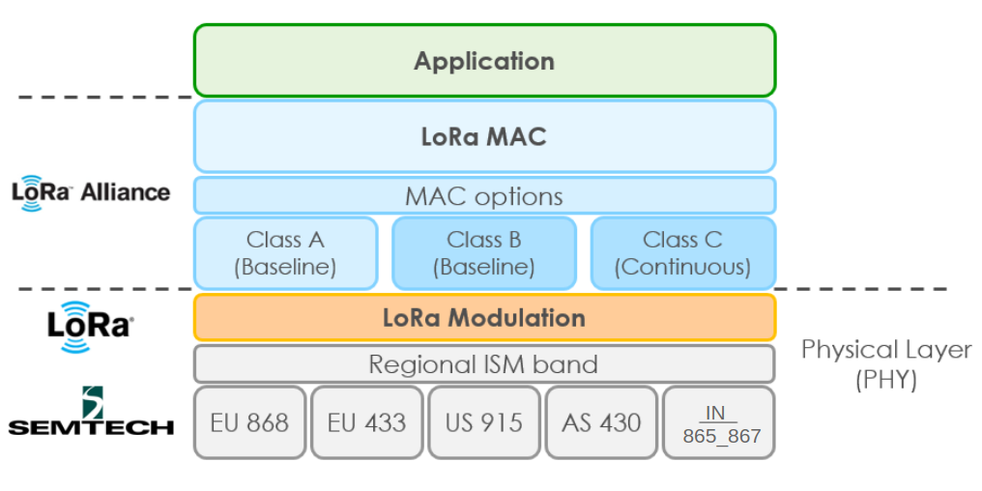
\includegraphics[width=0.7\linewidth]{images/lorawan/protocol_stack.png}
    \caption{LoRa technology model}
    \label{fig:stack}
\end{figure}

% What is LoRa
\section{Introduction to LoRa}
\label{lora}
LoRa, which stands for Long Range Radio, is an RF modulation technology for Low-Power Wide Area Networks (LPWANs). It is mainly targeted for M2M and IoT networks and enables public or multi-tenant networks to connect several applications running on the same network. Created by the French company Semtech \cite{8075570} to standardize LPWANs, LoRa grants long-range transmissions, going from five kilometers in urban areas to 15 kilometers in rural areas \cite{lora_developer_portal}.
\\
In detail, LoRa is a \textit{spread-spectrum} modulation technique. It derives from the existing Chirp Spread Spectrum (CSS) and operates in a fixed-bandwidth channel of either 125 kHz or 500 kHz for uplink channels and 500 kHz for downlink channels. The LoRa modulation ensures a trade-off between sensitivity and data rate. 
\\
Furthermore, LoRa uses orthogonal spreading factors to preserve the battery life of connected sensors by making adaptive optimizations of nodes' power levels and data rates.

\subsection{Key LoRa Modulation Properties}
These are the essential configuration parameters of LoRa radio
\begin{itemize}
    \item \textbf{Carrier Frequency} (CF): It is the frequency used for the communications from node to the gateway. LoRa operates at unlicensed frequency ISM bands 863-870 MHz in Europe and 915 MHz in U.S. \cite{7925650}.
    \item \textbf{Spreading Factory} (SF): It is the number of chirps per symbol. As reported in Table \ref{tab:spreading}, LoRa has 6 SF, whereas higher SFs allow larger coverage areas and, one symbol has 2 SF chirps for the overall frequency.

    % Please add the following required packages to your document preamble:
\begin{table}[h]
    \caption{Sensitivity of LoRa Receiver}
    \label{tab:spreading}
    \centering
    \begin{adjustbox}{max width=0.7\textwidth,center}
    \begin{tabular}{|l|llllll|}
    \hline
    \multicolumn{1}{|c|}{\multirow{2}{*}{\textit{BW}}} & \multicolumn{6}{c|}{\textbf{Spreading Factor}}                                                                                                                                                                           \\ \cline{2-7} 
    \multicolumn{1}{|c|}{}                             & \multicolumn{1}{c|}{\textit{SF7}} & \multicolumn{1}{c|}{\textit{SF8}} & \multicolumn{1}{c|}{\textit{SF9}} & \multicolumn{1}{c|}{\textit{SF10}} & \multicolumn{1}{c|}{\textit{SF11}} & \multicolumn{1}{c|}{\textit{SF12}} \\ \hline
    125 kHz                                            & \multicolumn{1}{l|}{-126.50}      & \multicolumn{1}{l|}{-127.25}      & \multicolumn{1}{l|}{-131.25}      & \multicolumn{1}{l|}{-132.75}       & \multicolumn{1}{l|}{-134.50}       & 133.25                             \\ \hline
    250 kHz                                            & \multicolumn{1}{l|}{-124.25}      & \multicolumn{1}{l|}{-126.75}      & \multicolumn{1}{l|}{-128.25}      & \multicolumn{1}{l|}{-130.25}       & \multicolumn{1}{l|}{-132.75}       & -132.25                            \\ \hline
    500 kHz                                            & \multicolumn{1}{l|}{-120.75}      & \multicolumn{1}{l|}{-124.00}      & \multicolumn{1}{l|}{-127.50}      & \multicolumn{1}{l|}{-128.75}       & \multicolumn{1}{l|}{-128.75}       & -133.25                            \\ \hline
    \end{tabular}
    \end{adjustbox}
\end{table}    

    \item \textbf{Bandwidth} (BW): LoRa has three bandwidth options: 125 kHz, 250 kHz, and 500 kHz. The 125 kHz bandwidth is used for the 863-870 MHz frequency band, the 500 kHz bandwidth for rapid transmissions, and the 125 kHz bandwidth to cover wide areas. The correlation among duration of symbol \(\ T_{s} \), the bandwidth \textit{BW}, and the spreading factor \textit{SF} is given by:
    
    \[\ T_{s} = \frac{2^{SF}}{BW} \]
    
    \vspace{0.5pt}
    
    \item \textbf{Coding Rate} (CR): LoRa adds a forward error correction (FEC) in every data transmission by encoding 4-bit data with redundancies into 5-bit, 6-bit, 7-bit, or even 8-bit. With this redundancy. the LoRa signal can endure short interferences. The Coding Rate (CR) value needs to be adjusted according to the conditions of the channel used for data transmission. In case of many interferences in the channel, it’s recommended to increase the value of CR, even if it also increases the duration of the transmission. Coding rate expression is \(\ CR = \frac{4}{4+n} \), where \(\ n \in \{1,2,3,4\} \). The modulation bit rate \(\ R_{b} \) is defined as:
    
    \[\ R_{b} = \frac{4}{4 + n}\frac{BW}{2^{SF}} \]
    
    \vspace{1pt}

\end{itemize}
These parameters impact the receiver sensitivity. As the bandwidth increases, the sensitivity of the decoder lowers. The decrease in code rate helps to reduce Packet Error Rate (PER) against interference. For example, a message transmitted with a 4/8 code rate is more resilient on channel implications than a message with a code rate of 4/5.

% architecture
\section{LoRaWAN network topology}
\label{topology}
Typically, IoT applications adopt a mesh architecture to increase communication ranges and cell sizes of the network. However, this approach can affect the device's battery life, as the nodes have to forward messages to each other \cite{article}. Conversely, to increase sensors' lifetime, the LoRaWAN network uses the simpler star-of-stars topology.  This architecture consists of the following elements:
\begin{figure}
    \centering
    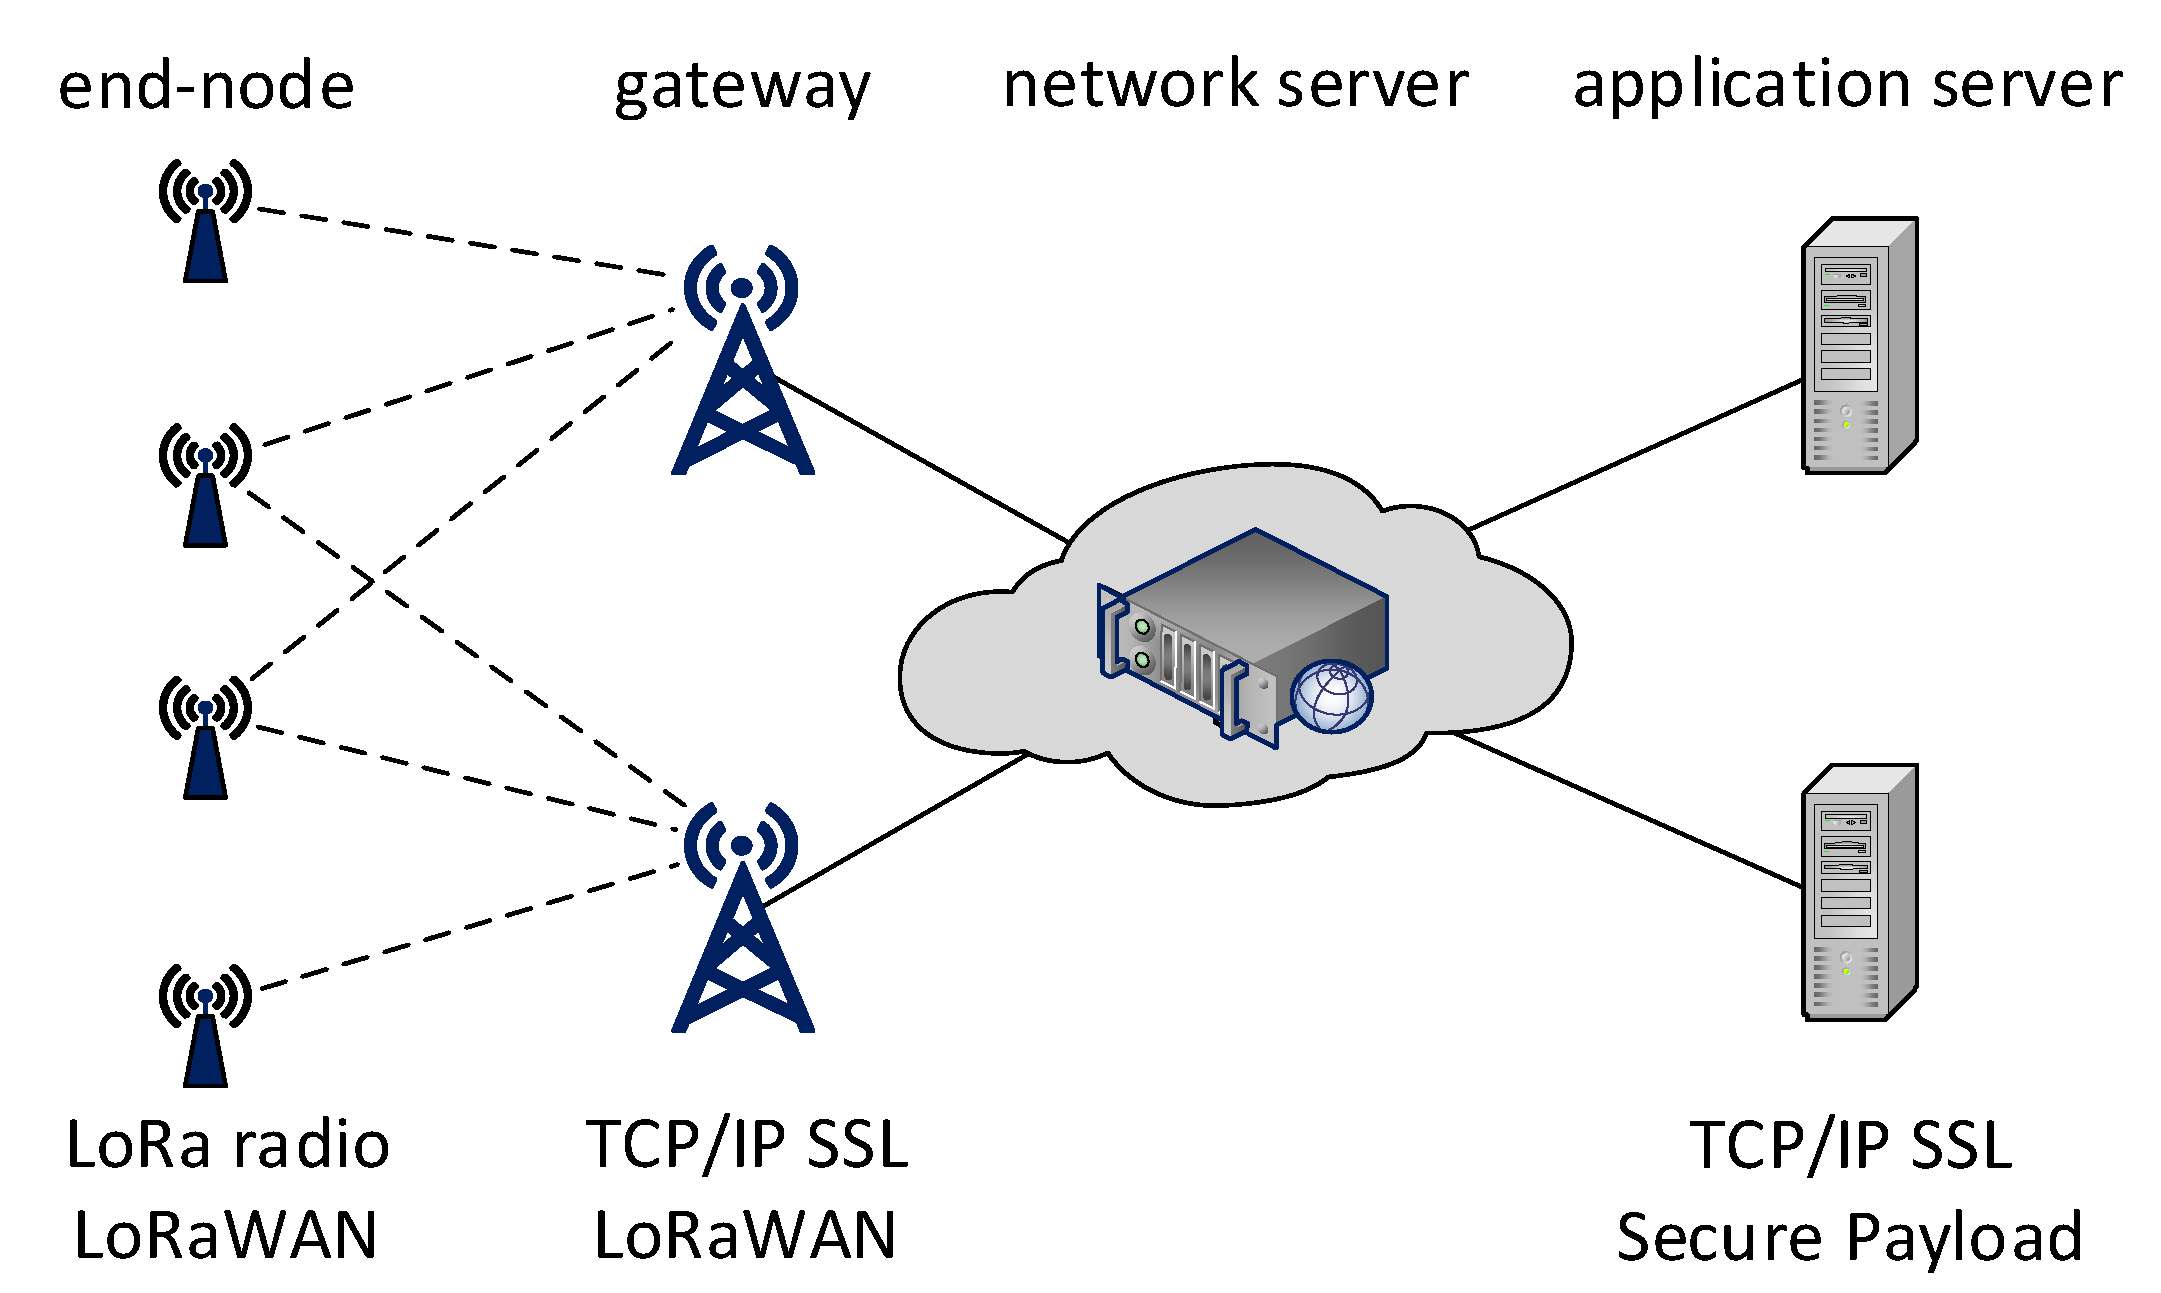
\includegraphics[width=0.7\linewidth]{images/lorawan/architecture.png}
    \caption{LoRaWAN architecture}
    \label{fig:architecture}
\end{figure}
\begin{itemize}
	\item \textbf{End Devices (EDs)}: low power sensors/actuators, battery operated. They are wirelessly connected to the network through gateways and use the LoRa RF modulation to communicate.
	\item \textbf{Gateway (GW)}: It receives messages from end devices and forwards them to the Network Server. A gateway connects to the Internet through an IP backbone.
	\item \textbf{Network Server (NS)}: This server manages the entire network. It receives IP traffic from gateways and is responsible for network management.
	\item \textbf{Application Server (AS)}: The application server processes messages received from end devices and generates downlink payloads to send to end devices. There may be more than one Application Server on the network
\end{itemize}
Since LoRaWAN networks use an ALOHA-based protocol, end devices don't need to be associated with a specific gateway for accessing the network. Consequently, the gateway acts simply like relays to which endpoints transmit data via the LoRa RF interface. On the other side, gateways forward the received packets to servers using the common IP networks such as 3G/4G, Ethernet, or WiFi.

\section{Device Classes}
\lorawan specifies three classes of devices: A, B, and C. These classes are distinguished by each other by the MAC procedures and by power consumption profiles. All devices implement Class A, whereas Class B and Class C extend the specification of Class A devices. Figures \ref{fig:classes} illustrate the three classes, defined as follow:

\begin{figure}
    \centering
    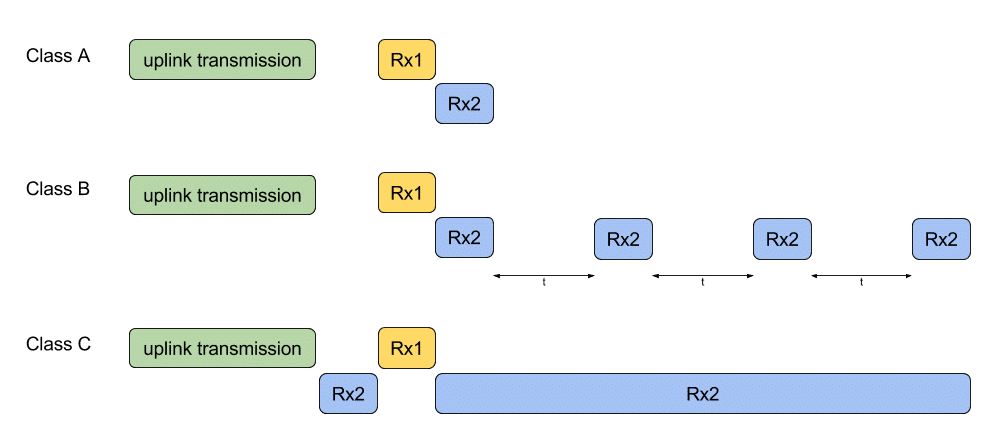
\includegraphics[width=0.7\linewidth]{images/lorawan/device_classes.png}
    \caption{The classes of LoRaWAN devices}
    \label{fig:classes}
\end{figure}

\begin{enumerate}

    \item \textbf{Class A} Class A devices support bi-directional communication. Both uplink and downlink transmission are done in the same randomly chosen radio channel. Every node observes the acknowledgment in receive windows, RX1 and RX2, during downlink transmission. Delays from the end of an uplink transmission to the start of receive windows (RX1 and RX2) are defined as Receive Delay 1 (RX1Delay) and Receive Delay 2 (RX2Delay, or RX1 + 1s).
    
    \item \textbf{Class B} Class B devices can open extra receiving slots at the scheduled times. The gateway generates a ping slot to integrate end devices to receive additional windows and broadcasts a time-synchronized periodic beacon to allow the Network Server (NS) to be aware of the listening status of end devices. Class B devices distribute the radio channel for downlink and uplink transmission to overcome the collision effect.
    
    \item \textbf{Class C}: Devices operating in Class C have the receive windows almost always open (they close the window only when they transmit). For this reason, Class C devices require more power to operate than Class A or Class B. In turn, they have the lowest latency for communication.
    
\end{enumerate}


\section{Frame format}
\begin{figure}[H]
    \centering
    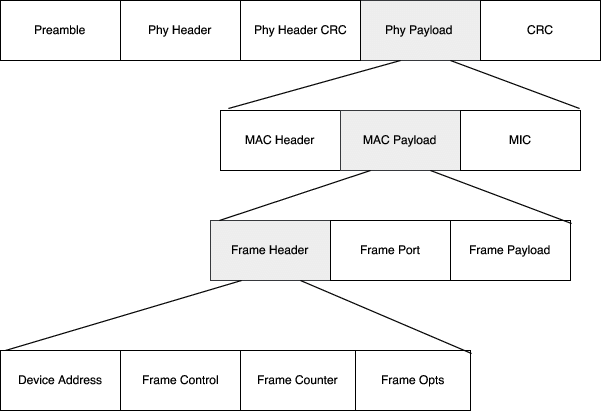
\includegraphics[width=0.7\linewidth]{images/lorawan/frame_format.png}
    \caption{}
    \label{fig:frame}
\end{figure}
The LoRaWAN frame, shown in \ref{fig:frame}, is structured as follows:
\begin{enumerate}
	\item \textit{Physical Layer}.  It has a preamble, that defines the modulation scheme, followed by a header and a payload. The header contains information such as payload length and whether the Payload 16-bit CRC is present in the frame (only uplink frames contain payload CRC). The payload contains the MAC frame.
	\item \textit{MAC Layer}. It consists of a header, a payload, and a Message Integrity Code (MIC). The header defines protocol version and message type, the payload contains the application data, and the MIC, computed using the header and the payload portions, is used to prevent the forgery of messages and authenticate the end node.
	\item \textit{Application Layer}. It consists of a header, a port, which value depends on the application type, and the payload. The header contains information about the device and the network and commands used to change parameters such as the data rate or the transmission payload. The payload contains the transmitted data and is encrypted with the AES 128 algorithm. 
\end{enumerate}


\subsection{Message types}
LoRaWAN message types transport MAC commands and application data. These messages are categorized into two main families, uplink and downlink messages, based on the direction they travel \cite{the_things_network_2021}:
\begin{enumerate}
	\item Uplink messages are sent by ED to the Network Server, relayed by one or many gateways.
	\item Each downlink message is sent by the Network Server to one ED and is relayed by a single gateway.
\end{enumerate}
LoRaWAN v1.1 defines several MAC message types, presented in the Table \ref{tab:message_types}. These messages are identified by the first bytes of the LoRaWAN packet, in the MHDR field, and specifically in a section of three bites, called \textit{MType}.
\begin{table}[H]
    \caption{MAC message types that can be found in LoRaWAN 1.1}
    \label{tab:message_types}
    \centering
    \begin{tabular}{|c|l|}
        %\toprule
        \hline
        \textbf{MType} & \textbf{Description}      \\ \hline
        000            & Join Request              \\ \hline
        001            & Join Accept               \\ \hline
        010            & Unconfirmed Data Up       \\ \hline
        011            & Unconfirmed Data Down     \\ \hline
        100            & Confirmed Data Up         \\ \hline
        101            & Confirmed Data Down       \\ \hline
        110            & Rejoin-request            \\ \hline
        111            & Proprietary               \\ \hline
        %\bottomrule   
    \end{tabular}
\end{table}
\begin{enumerate}
	\item Join Request, Join Accept and Re-Join are three messages used to establish a connection between the LoRa End Device and Network Server.
	\item Confirmed Data are data messages that need to be acknowledged by the receiver.
	\item Unconfirmed Data are data messages that do not require any acknowledgment.
	\item Proprietary messages are used to incorporate non-standard message format functionalities.
\end{enumerate}

\subsubsection{Addressing}
Each device has a global address, the \textit{\de}. It is a unique EUI64 identifier supplied by the manufacturer, stored in non-volatile memory, and used as a MAC address. The first 3 bits represent the Organizationally Unique Identifier (OUI), purchased from IEEE that represents the constructor.
\begin{figure}[H]
    \centering
    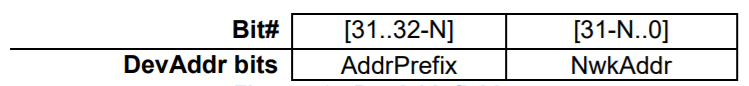
\includegraphics[width=0.7\linewidth]{images/lorawan/devaddr.PNG}
    \caption{DevAddr fields}
    \label{fig:devaddr}
\end{figure}
In addition, the LoRaWAN specification defines the \textit{DevAddress}, a dynamic 32-bit temporary address generated directly by the Network Server. As shown in Figure \ref{fig:devaddr}, The first significant bits represent the \textit{AddrPrefix}. It derives from NetID, the NS unique identifier attributed directly by the LoRa-Alliance to network providers and used in routing messages in the correct network. AddrPrefix describes the Network Server that is currently managing the device. The least significant bits define the \textit{NwkAddr}, the network address of the ED, set by the network manager.
\\
Network Servers know for each device the unique DevEUI and the current DevAddress.

\section{Device Activation}
A LoRa device, to send and receive messages in the network, needs to be registered in the network, following a procedure called \textit{activation}. Before the activation, three parameters of the device should be configured: the \textit{AppEUI}, the \textit{DevEUI}, and \textit{AppKey} (an AES-128 bit secret key known as the root key). The activation procedure generates the \textit{DevAddress} and two session keys, \textit{nwkSKey} and \textit{appSKey}, used to encrypt and transmit packets to the server. \lorawan offers two different activation methods: Over-the-Air Activation (OTAA) and Activation by Personalization (ABP). Since OTAA is more securer and more flexible than ABP, it is the recommended process for activation for LoRaWAN \cite{the_things_network}.

\subsection{Over-the-Air Activation}
Devices perform a join procedure with the network to receive a dynamic device address and negotiate security keys. This procedure requires the exchanging of two MAC messages between the end device and the Network Server:
\begin{itemize}
	\item \textit{\jr}, from the ED to the Network Server.
	\item \textit{\ja}, from the Network Server to the ED.
\end{itemize}
The end device initializes the join procedure, which sends to the network the Join-request message, composed of the following fields: \textit{JoinEUI}, an IEEE EUI64 address that uniquely identifies the Join Server, the \textit{DevNonce}, a 2-byte counter, used to prevent replay attacks, and the \textit{DevEUI} global identifier. 
\begin{figure}
    \centering
    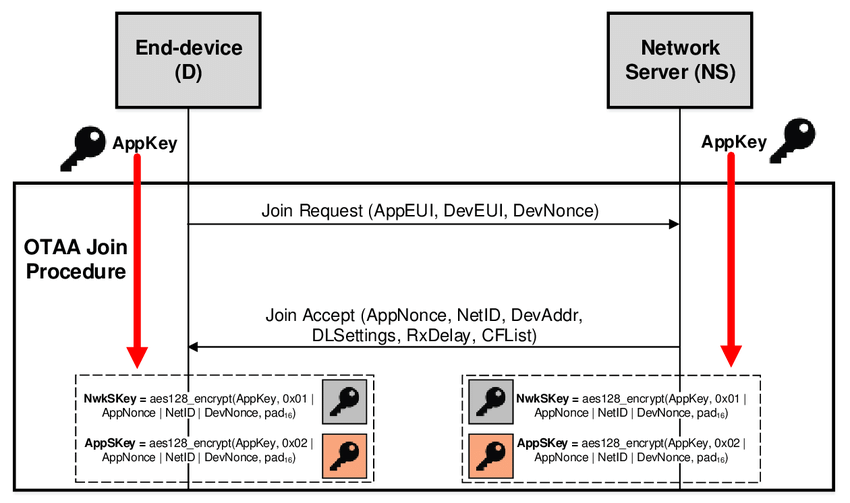
\includegraphics[width=0.9\linewidth]{images/lorawan/OTAA.png}
    \caption{OTAA message flow}
    \label{fig:otaa}
\end{figure}
The Network Server processes the request message and generates the Join-accept message. The main fields of the Join-accept are the \textit{NetID}, a network identifier, the \textit{JoinNonce}, a device-specific counter value used to calculate the session keys, and finally, the \textit{DevAddr}. The Join-accept message, encrypted using AES in ECB mode, is sent to the end device, now allowed to register in the network.

\subsection{Activation by Personalization}
Activation By Personalization (ABP) directly ties an end device to a pre-selected network. Devices and Network Server stores directly the \da and the two session keys NwkSKey and AppSKey instead of the \de, AppEUI, and the AppKey (each end device should have a unique set of NwkSKey and AppSkey). Although this activation procedure is easier than OTAA, it is less secure. To switch the network, devices have to manually change the keys. Moreover, they keep the same security session for their entire lifetime. 